\section{x-commerce architecture}
\label{sec:x_commerce_architecture}
A Web application developed by using the x-commerce toolkit, is a full stack JavaScript Single Page Application.
\begin{figure}[htb]
\centering
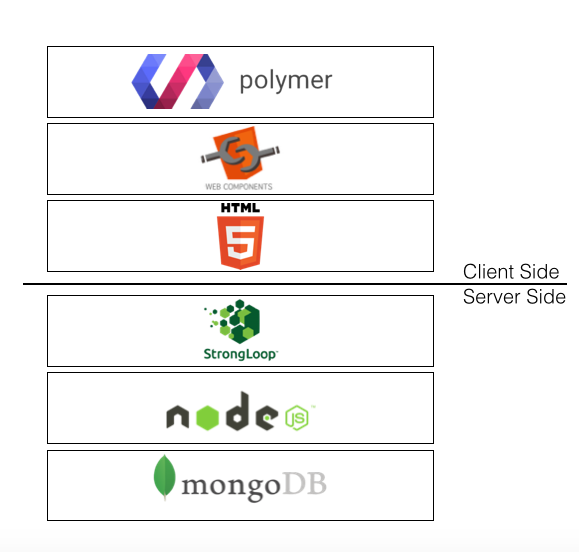
\includegraphics[width=0.7\linewidth]{images/chapter4/XPR_stack.png}\hfill
\caption[X-commerce architecture]{X-commerce architecture}
\label{fig:x_commerce_architecture}
\end{figure}
\subsection{server side}
On the server side, an x-commerce application is based on NodeJS (see \ref{sec:nodejs}) used to create the server environment, MongoDB (see \ref{sec:mongodb}) used to store data, and the Web framework Loopback by Strongloop (see \ref{sec:strongloop_loopback}).
\newline
Node.js is a JavaScript runtime built on Chrome’s V8 JavaScript engine. Node.js uses an event-driven, non-blocking I/O model that makes it lightweight and efficient. Node.js package ecosystem, npm, is the largest of such a kind of open source libraries in the world. NodeJS lets to create a vertical full-stack application in Javascript. The NodeJS asynchronous development scheme increases performances of web applications, by using downtime caused by HTTP requests.
\newline
LoopBack generates model API from the model schemas, to let CRUD operations on models. Loopback is the core of the X-commerce server-side. Document oriented API definition guarantees easiness and speed in API creation. Moreover, Loopback, is fully compatible with several DBMS thanks to connectors.
\newline
MongoDB is a cross-platform document-oriented database. Classified as a NoSQL database, MongoDB eschews the traditional table-based relational database structure in favor of JSON-like documents with dynamic schemas. The document-oriented being of MongoDB allows to horizontal scale in really easy way. Moreover, document models, that replace relational database’s rows, are schemaless: this feature gives to MongoDB project high levels of felxibility and manageability.
\subsection{client side}
On the client side, an x-commerce application is based on HTML5 Web Components via Polymer-Project by Google. It is a set of Polymer elements for local routing, API request, forms, lists, style and administrator panels.
\newline
Polymer-Project is one of the most important emerging realities of the time. Google team has heavily focused it's forces on code reusability and on separation between behavior, presentation and content. Code reusability is a direct effect of Web Components structure: the creation of widget that can be completely indipendent facilitates code reuse.
\newline
Finally, the union between Polymer and Strongloop has been topped by the creation of the document oriented development process described below \ref{sec:document_driven_web_development_process}.